\documentclass[tikz,border=2pt]{standalone}
\usepackage{amsmath}
\usepackage{pgfplots}
\pgfplotsset{compat=1.18}
\usetikzlibrary{arrows.meta}
\begin{document}
% Study-hours example: v(a) = 12a - a^2 on A = [0,10]; the rational choice a* = 6 attains
% v(6) = 36, so v(a*) >= v(a) for every a in A (the whole graph lies below the line v = 36).
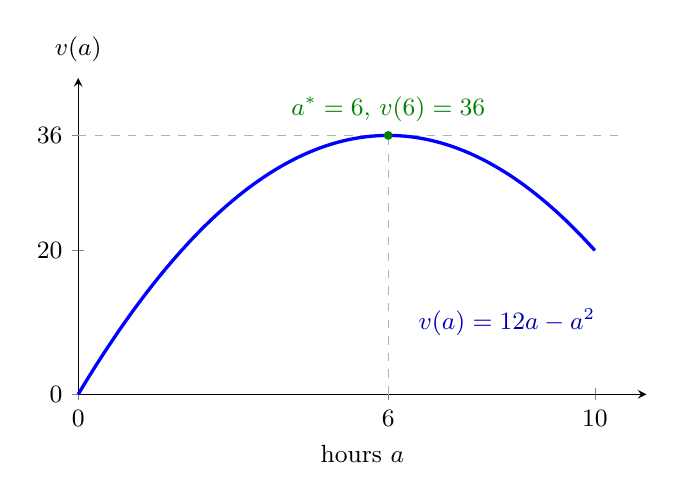
\begin{tikzpicture}[font=\small, >={Latex[length=2mm]}]
  \begin{axis}[
    axis lines=left, xmin=0, xmax=11, ymin=0, ymax=44,
    xtick={0,6,10}, ytick={0,20,36},
    xlabel={hours $a$}, ylabel={$v(a)$},
    ylabel style={rotate=-90, anchor=south, at={(axis description cs:0,1.02)}},
    width=8.8cm, height=5.6cm, clip=false, samples=80, smooth]
    \addplot[gray!60, thin, dashed, domain=0:10.6, samples=2] {36};
    \addplot[gray!60, thin, dashed] coordinates {(6,0) (6,36)};
    \addplot[blue, very thick, domain=0:10] {12*x-x^2};
    \fill[green!50!black] (axis cs:6,36) circle (1.6pt);
    \node[green!50!black, anchor=south] at (axis cs:6,36.6) {$a^*=6$, $v(6)=36$};
    \node[blue!70!black, anchor=west] at (axis cs:6.4,10) {$v(a)=12a-a^2$};
  \end{axis}
\end{tikzpicture}
\end{document}
